\documentclass{article}
\usepackage[utf8]{inputenc}
\usepackage{amssymb}
\usepackage{mathtools} 
\usepackage{geometry}
 \geometry{
 a4paper,
 total={140mm,227mm},
 left=35mm,
 top=35mm,
 }

\usepackage{float}
\usepackage{graphicx}
\usepackage{epstopdf}
\usepackage{amsmath}
\usepackage{bm}

\setlength{\parindent}{0pt}
\numberwithin{figure}{section}
% equation number format: in section 1, (1.1), (1.2) ..
\usepackage{amsmath}
\usepackage{ dsfont }
\numberwithin{equation}{section}

\makeatletter
% we use \prefix@<level> only if it is defined
\renewcommand{\@seccntformat}[1]{%
  \ifcsname prefix@#1\endcsname
    \csname prefix@#1\endcsname
  \else
    \csname the#1\endcsname\quad
  \fi}
% define \prefix@section
% \newcommand\prefix@section{}
\makeatother

%% multi col
\usepackage{multicol}

% hyperlinks
\usepackage{hyperref}
\hypersetup{
    colorlinks=true,
    linkcolor=black,   
    urlcolor=black,
    filecolor=black,
} 
\urlstyle{same}

% colored frames (boxes)
\usepackage{xcolor}
\usepackage{mdframed}

% vector arrow with \vv{ }
\usepackage{esvect}

%\hyphenpenalty 10000
%\exhyphenpenalty 10000
%\usepackage[none]{hyphenat}
%\usepackage[document]{ragged2e}

% strike through text
\usepackage[normalem]{ulem}
% \sout{Hello World}
\title{A1 Diskret Matematik}
\author{Roar Nind Steffensen (s144107) & Magnus Middelboe Søborg-Madsen (s144063)}
\date{September 2016}

\begin{document}
\maketitle
\section{Opgave A}

a) Den givne formel er skrevet og løst på tableau form:

\begin{figure}[H]
    \centering
    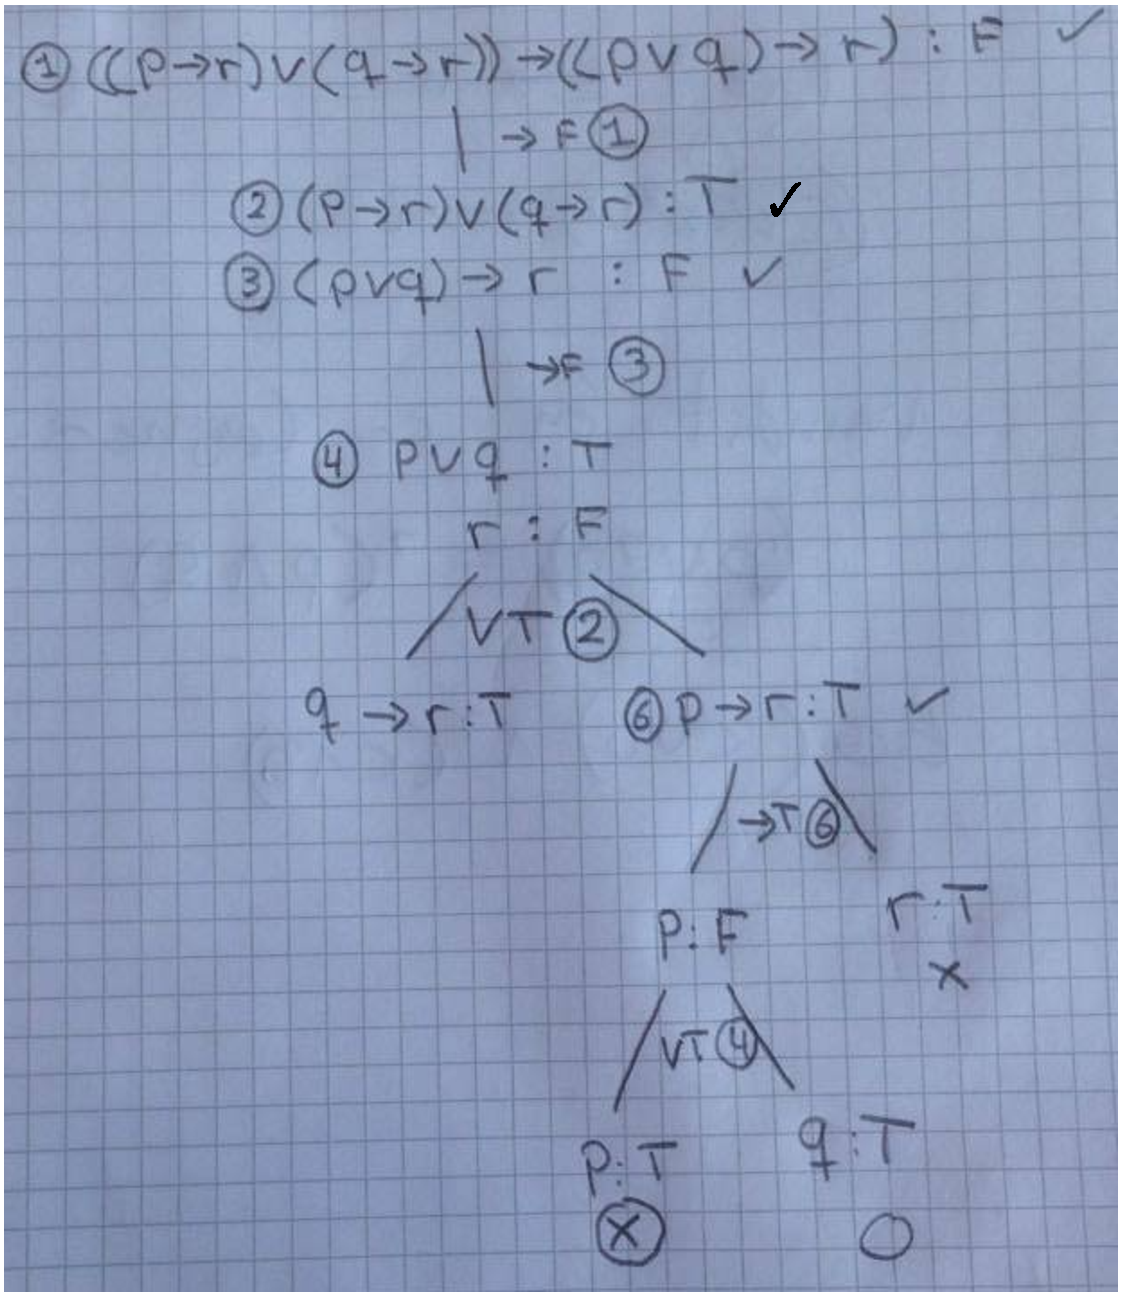
\includegraphics[height=13 cm]{OpgA/tableauAa2.pdf}
    \label{fig:Aa}
\end{figure}

Da en gren fandtes mættet og åben, er formlen opfyldelig med sandhedstildelingen
\begin{equation*}
    r:\text{F},\: p:\text{F}, \: q: \text{T}
\end{equation*}

Man kan vha. en sandhedstabel vise, at også sandhedstildelingen $p:\text{T},\: q:\text{F}, \: r: \text{F}$ er en løsning. Opgaveformuleringen spurgte dog specifikt om tableau-metoden, og bad os om ikke at fortsætte, når vi fandt blot en enkel åben mættet gren.
\newpage
b) Den givne formel er skrevet og løst på tableau form:

\begin{figure}[H]
    \centering
    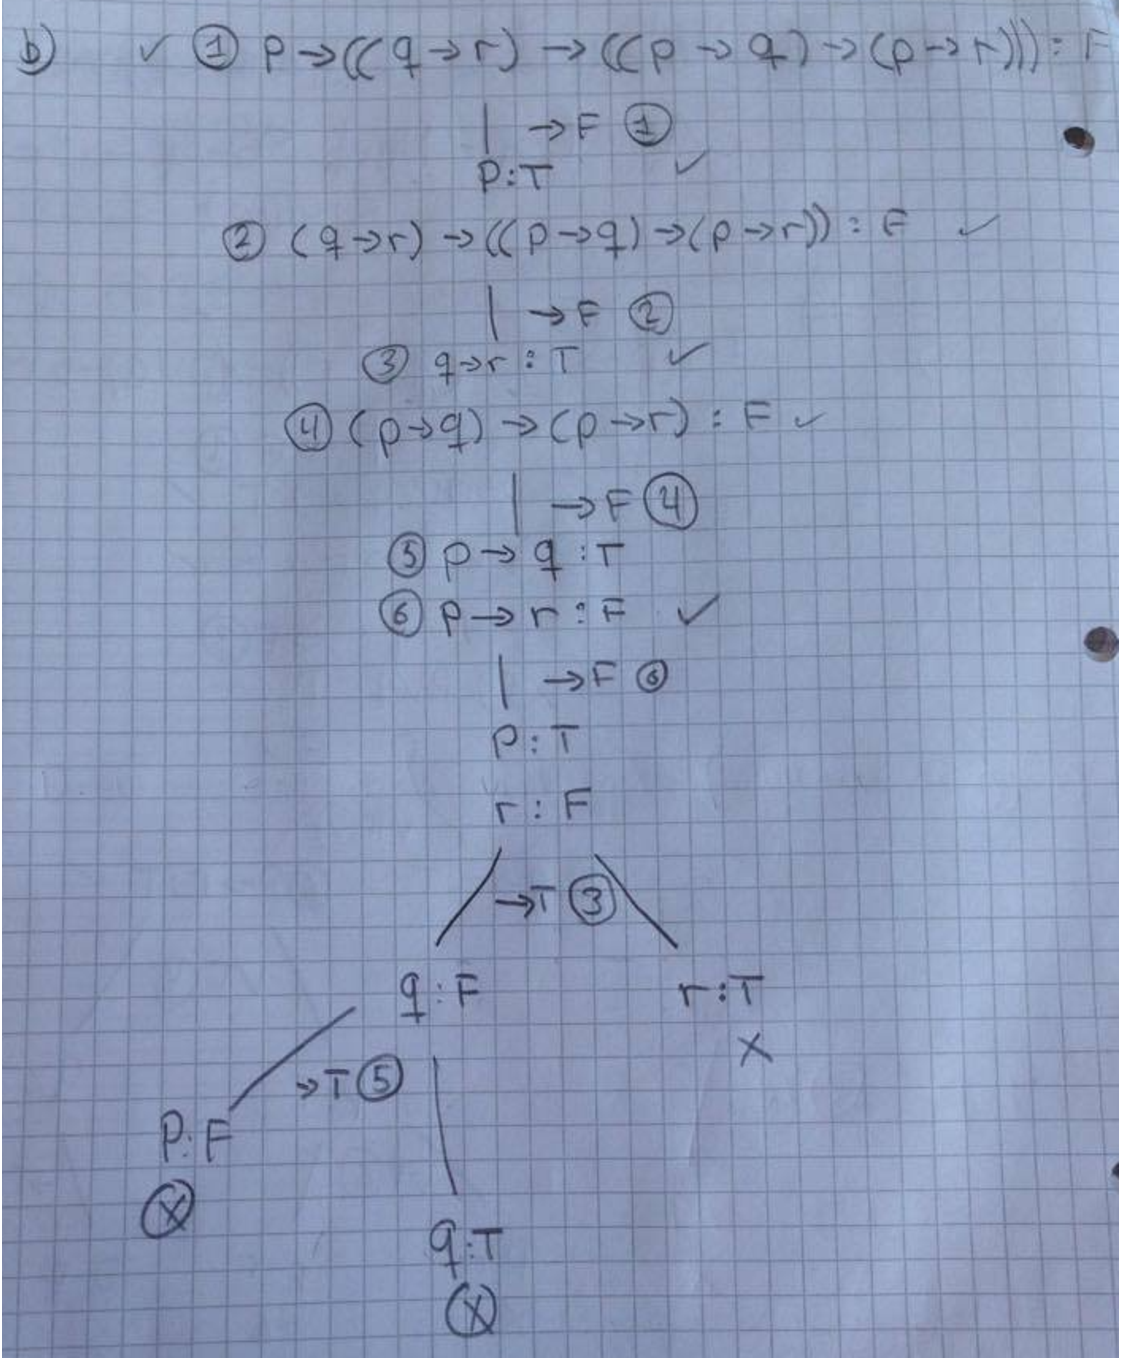
\includegraphics[height=13 cm]{OpgA/tableauAb.pdf}
    \label{fig:Ab}
\end{figure}

Da alle grene er lukkede, er formlen dermed gyldig.

\section{Opgave B}
Følgende slutning er givet: \\

\begin{figure}[H]
    \centering
    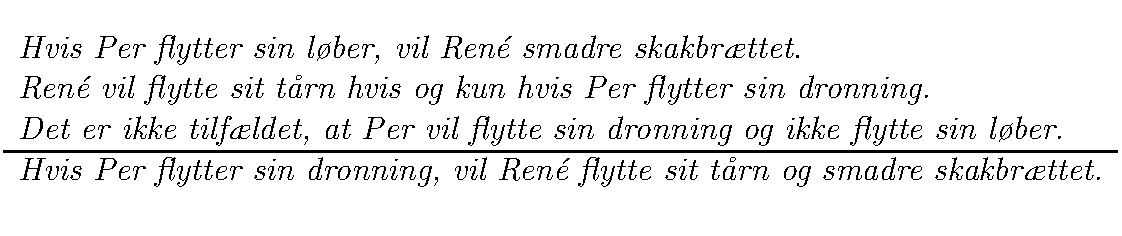
\includegraphics[width=0.9\textwidth]{OpgB/opgaveB.pdf}
    \label{fig:B}
\end{figure}

Først tildeler vi udsagnene nogle prædikatsymboler. \\

$l$: Per flytter sin løber. $s$: René smadrer skakbrættet. $t$: René flytter sit tårn. $d$: Per flytter sin dronning. \\

Herfra kan vi skrive slutninge som: 

\begin{align*}
    &l \rightarrow s \\
    &t \leftrightarrow d \\
    &\neg (d \wedge \neg l) \\
    &\rule{2cm}{0.4pt}\\
    &d \rightarrow (t \wedge s)
\end{align*}

For at slutningen er sand, skal konklusionen være sand antaget at hvert præmis er sandt. Dette kan tjekkes på tableau form:

\begin{figure}[H]
    \centering
    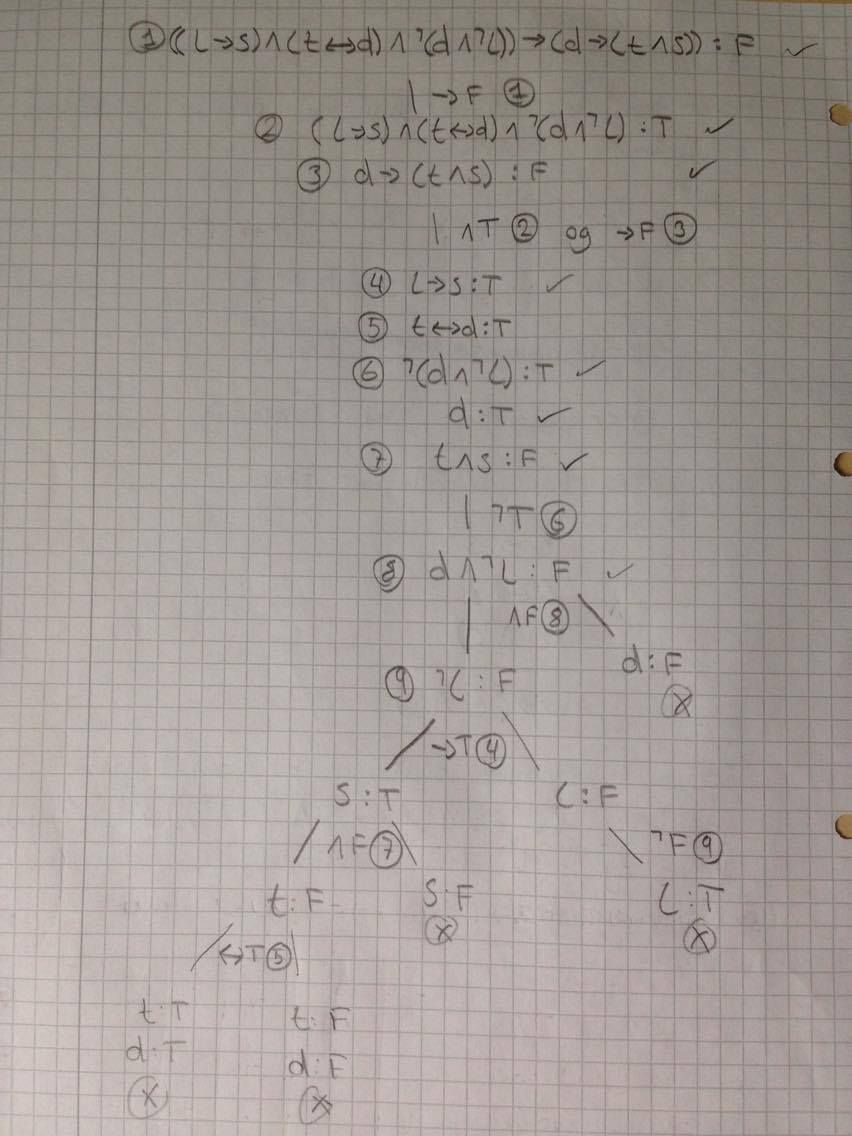
\includegraphics[width=0.8\textwidth]{OpgB/tableauB.jpg}
    \label{fig:B}
\end{figure}

Alle grene er mættede og lukkede svarende til at formlen er gyldig og slutningen er dermed logisk korrekt.

\section{Opgave C}
To unære prædikater $S$ og $Æ$ er givet, samt fortolkningen $\mathcal{F}$. \\

dom($\mathcal{F}$) $=$ alle mennesker.\\
$S^{\mathcal{F}}=$ \_ er studerende. \\
$Æ^{\mathcal{F}}=$ \_ er ærlig. \\
\\
Følgende sætninger er oversat til prædikatlogik under fortolkningen $\mathcal{F}$:\\
\\
a) Alle studerende er ærlige:\\
    $$\forall x(S(x) \rightarrow Æ(x))$$

b) Alle studerende er uærlige:\\
    $$\forall x(S(x) \rightarrow \neg Æ(x))$$
    
c) Ikke alle studerende er ærlige:\\
    $$\neg\forall x(S(x) \rightarrow Æ(x))$$
    
d) Ikke alle studerende er uærlige:\\
    $$\neg\forall x(S(x) \rightarrow \neg Æ(x))$$
    
d) Nogen studerende er ærlige:\\
    $$ \exists x(S(x) \wedge Æ(x))$$

f) Nogen studerende er uærlige:\\
    $$ \exists x(S(x) \wedge \negÆ(x))$$
    
g) Ingen studerende er ærlige:\\
    $$ \neg\exists x(S(x) \wedge Æ(x))$$
    
h) Ingen studerende er uærlige:\\
    $$ \neg\exists x(S(x) \wedge \negÆ(x))$$
    
Vi kan se, at fx. udtrykket i g) og i b) indeholder samme information, hvilket antyder at man kan gå fra en alkvantor til en eksistenskvantor ved at negere udtrykket (samt forholde sig til $\rightarrow$ og $\wedge$).

\section{Opgave D}
Følgende udtryk er oversat og analyseret fra prædikatlogik under fortolkningen $\mathcal{R}$:\\

dom($\mathcal{R}$)$=$ de reelle tal.\\
De anvendte matematiske symboler har konventionel betydning i fortolkningen $\mathcal{R}$. \\
\\
1) $\forall x(x=x^2 \rightarrow x < 0)$:
\begin{center}
Alle reelle tal, hvor tallet er lig tallet selv kvadreret, er negative.
\end{center}
\hspace{7 cm} - Nej, da $0 = 0^2$ og $1=1^2$. \\

\newpage
2) $\forall x(x>0 \rightarrow x^2 > x)$:
\begin{center}
Alle reelle positive tal kvadreret, er større end tallet selv.
\end{center}
\hspace{7 cm} - Nej, da $1 \nless 1^2$.  \\

3) $\forall x(x=0 \vee \neg(x+x=x))$:
\begin{center}
Alle reelle tal er enten nul eller ulig det dobbelte af tallet selv, dvs. $x=0$ eller $2x \ne x$.
\end{center}
\hspace{7 cm} - Ja, da kun $0$ er løsning til $2x=x$.  \\

4) $\exists x\forall y(x>y)$:
\begin{center}
%For et hvert reelt tal findes der et andet større reelt tal.
Der findes et reelt tal, som er større end alle reelle tal.
\end{center}
%\hspace{7 cm} - Ja, da $\infty$ ikke er del af $\mathds{R}$.  \\
\hspace{7 cm} Nej, da $\infty$ ikke er del af $\mathds{R}$.

5) $\forall x\forall y(x>y \rightarrow \exists z(x>z \wedge z>y))$:
\begin{center}
For alle reelle talpar, hvor det ene tal er større end det andet,\\ findes et tredje reelt tal med en værdi mellem de to.
\end{center}
\hspace{7 cm} - Ja. Der er ingen grænse for decimaler i $\mathds{R}$. Det er altid muligt at finde et reelt tal i intervallet $]x,y[$ for $y>x$.

\section{Opgave E}
Opgaven er givet ved, at der findes 2 typer af mennesker på en ø. Sandsigere som \textbf{altid} siger sandheden, og Løgnere som \textbf{altid} lyver. Ellers er menneskene identiske.\\
\\
a) Opgaven lyder:

\begin{center}
\textit{Engang besøgte en fremmed øen. Der mødte han to af øens indbyggere, Peter og Signe. Han spurgte dem: “Er nogen af jer en løgner?”. “Mindst en af os er løgner”, svarede Peter. Hvad er Peter og Signe (sandsigere eller løgnere)?}
\end{center}

Vi tildeler følgende prædikatsymboler:\\
$p$: Peter er sandsiger.\\ $s$: Signe er sandsiger.\\
\\
Udsagnet kan dermed skrives som formlen: 

\begin{equation}
p \leftrightarrow \neg (p \wedge s)
\label{eq:E1}
\end{equation}

Ved at stille en sandhedstabel op, kan vi se hvilken sandhedstildeling der tilfredstiller udsagnet.

\begin{table}[H]
\centering
\begin{tabular}{c|c|c}
$p$ & $s$ & Formel \eqref{eq:E1} \\ \hline
T & T & F  \\
T & F & T  \\
F & T & F  \\
F & F & F 
\end{tabular}
\end{table}

Det kan konstateres at Peter er en sandsiger og Signe er en løgner.\\
\\
\\

b) Opgaven lyder: 

\begin{center}
\textit{Mens den fremmede vandrede rundt på øen mødte han to andre indbyggere, Anne og Bob. Han spurgte Anne: “Er nogen af jer en sandsiger?”. “Hvis Bob er en løgner, så er jeg også en løgner”, svarede Anne. Hvad er Anne og Bob?}
\end{center}

Ligesom før tildeles der prædikatsymboler:\\
$a$: Anne er sandsiger. \\
$b$: Bob er sandsiger. \\
\\

Udsagnet kan dermed skrives som formlen: 

\begin{equation}
a \leftrightarrow (\neg b \rightarrow \neg a)
\label{eq:E2}
\end{equation}

Igen kigger vi på sandhedstabellen:

\begin{table}[H]
\centering
\begin{tabular}{c|c|c}
$a$ & $b$ & Formel \eqref{eq:E2} \\ \hline
T & T & T  \\
T & F & F  \\
F & T & F  \\
F & F & F 
\end{tabular}
\end{table}

Vi ser at udsagnet kun går op, hvis både Anne og Bob er sandsigere.\\
\\

c) Opgaven lyder:

\begin{center}
\textit{Den fremmede vandrede videre. Om aftenen begyndte han at søge efter ly for natten, men var meget forsigtig, for han vidste at nogen af øens indbyggere var kannibaler, og det var ikke muligt at skelne dem ved deres udseende. Han mødte så tre af øens indbyggere, Carsten, Diana og Erika. Han spurgte Carsten: “Hvor mange af jer er sandsigere?”. “Flam flim”, svarede Carsten på sit eget sprog. “Hvad sagde han?”, spurgte den fremmede Diana. Han sagde “Kun én”, svarede Diana. “Stol ikke på Diana, hun er en løgner. Kom med mig, jeg er ikke en kannibal”, sagde Erika. “Nej, kom med mig, jeg er ikke en kannibal”, sagde Diana. Hvad skal den fremmede gøre?}
\end{center}

Prædikatsymboler tildelt: \\
$d$: Diana er sandsiger. \\
$c$: Carsten er sandsiger.\\
$e$: Erica er sandsiger.\\
\\

De første to udsagns skrives ved formlerne: 

\begin{gather}
    d \leftrightarrow ( c \leftrightarrow ( e \oplus (c \vee d) \wedge \neg (c \wedge d))) \label{eq:E3a} \\ 
    e \leftrightarrow \neg d  \label{eq:E3b}
\end{gather} 

Den komplekse højreside i formel \eqref{eq:E3a} kommer fra udsagnet "kun én". Det kan se lidt svært ud, men det er let at tjekke. \\
Idéen med fx $d \leftrightarrow (\text{Dianas udsagn})$ er, Dianas udsagn er sandt, hvis og kun hvis Diana er sandsiger. Erika og Diana benægter hinandens udsagn, derfor $e \leftrightarrow \neg d$. Sandhedstabellen kommer til at se ud som følgende:

\begin{table}[H]
\centering
\begin{tabular}{c|c|c|c|c|c}
d & c & e & Formel \eqref{eq:E3a} & Formel \eqref{eq:E3b} & Formel \eqref{eq:E3a} $\wedge$ Formel \eqref{eq:E3b}\\ \hline
T & T & T & F      & F  & F \\
T & T & F & F      & T  & F\\
T & F & T & T      & F  & F   \\
T & F & F & F      & T  & F    \\
F & T & T & T      & T  & T    \\
F & T & F & F      & F  & F    \\
F & F & T & T      & F  & F    \\
F & F & F & F      & F  & F   
\end{tabular}
\end{table}

På samme måde som tidligere, ser vi at der kun er én sandhedstildeling der tilfredsstiller begge udsagn (formlerne \eqref{eq:E3a} og \eqref{eq:E3b}). Altså må Diana være en løgner, mens Carsten og Erika er sandsigere.\\
\\
Fra de sidste udsagn i opgaven ser vi, at Diana er en kannibal, og at den fremmede skal følge med Erika som ikke er kannibal.


\end{document}
